In der Abbildung $\ref{fig.bild}$ wird ein typisches Signalbild dargestellt.
Auf der X-Achse wird das Magnetfeld aufgetragen, auf der Y-Achse die Transparenz des Mediums.
Das Minimum auf der linken Seite entsteht dadurch, dass dort kein Magnetfeld anliegt uns es so auch zu keiner Zeemanaufspaltung kommen kann.
Die anderen beiden Minima enstehen durch die gegebenen Isotope $R_{87}$ und $R_{85}$.
Im folgenden wird die Zuortnung der Isotote zu den Minima vorgenommen.
Bis zu dem Zeitpunkt werden die Minnima mit 1 und 2 (von Links nach Rechts) bezeichnet.
\begin{figure}[h!]
  \centering
  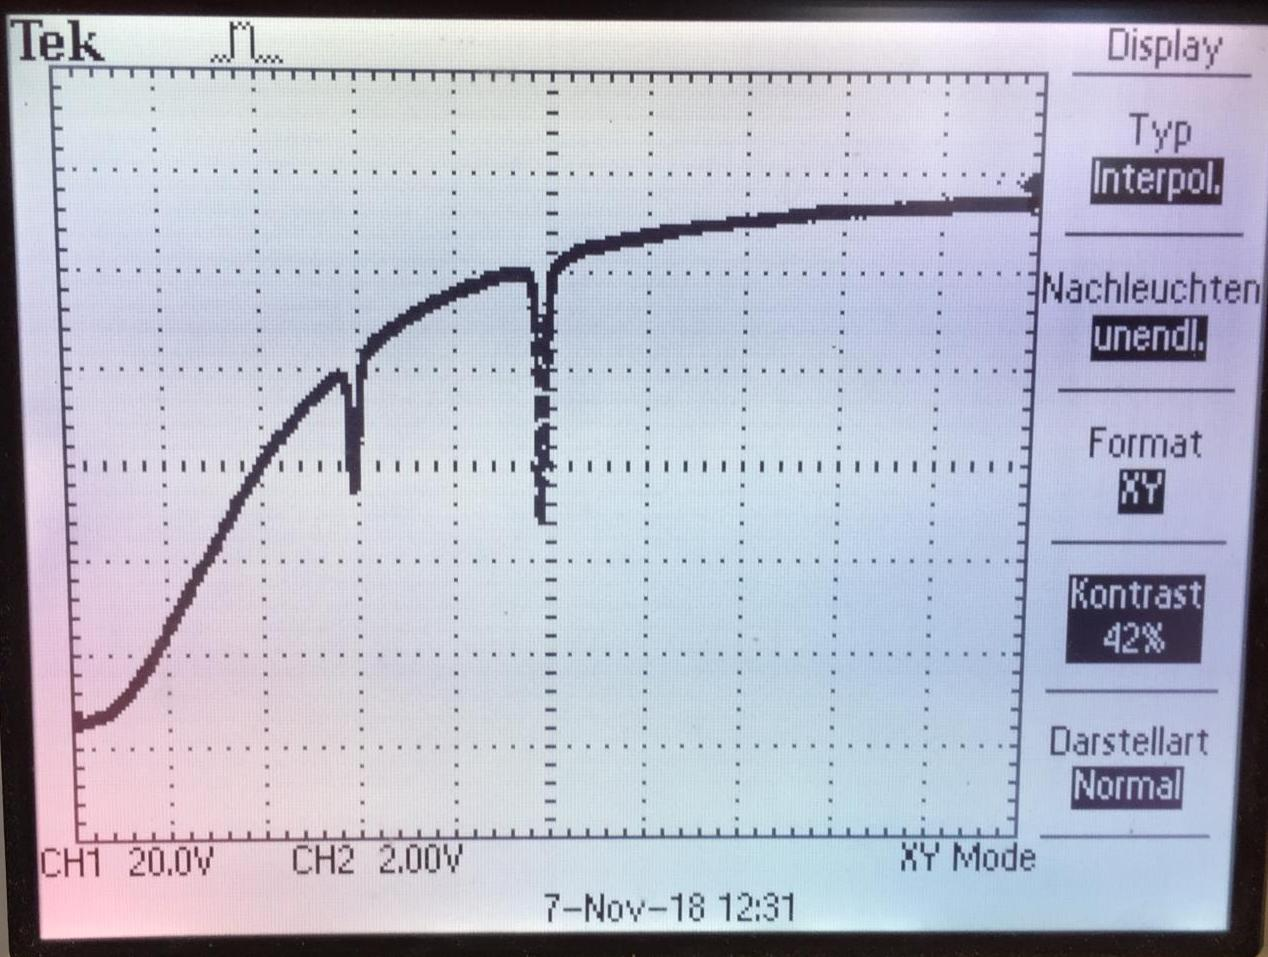
\includegraphics[width=0.8\textwidth]{bild.jpeg}
  \caption{Das für die Resonanzstelle benötigte Magnetfeld aufgetragen auf die Frequenz}
  \label{fig.bild}
\end{figure}
Anhand der Abbildung $\ref{fig.bild}$ kann eine Abschätzung des Verhältnisses der beiden Isotope getroffen werden.
Dabei gilt:
\begin{align*}
  N_1+N_2 = 1
\end{align*}
N beschreibt dabei den prozentualen Anteil an der Gesamtanzahl.
Durch Ausmessen der Minima ergibt sich ein Verhältniss $R$ für $\frac{\text{Isotop 1}}{\text{Isotop 2}}$ von:
\begin{align*}
  R=\SI{0.48}{}
\end{align*}
\begin{align*}
  N_1&=\frac{0,48}{1+0,48}=0,32\\
  N_2&=1-N_1=0,68
\end{align*}


Um die Resonanzstellen zu erreichen können die Potentiometer für die Horizontale Spule und für die Sweep-Spule variiert werden.
Die zur jeweiligen Resonanzstelle gehörigen Potentiometerumdrehungen können wie folgt in einen Stromstärke umgerechnet werden.
\begin{align*}
  \text{Sweep-Spule}&&&\text{Horizontale Spule}\\
  1 \text{Umdrehung} &= \SI{0,1}{A}&&1 \text{Umdrehung} = \SI{0,3}{A}
\end{align*}
Aus den resultierenden Stromstärken kann das B-Feld berrechnet werden.
\begin{align*}
  B=\mu_0\frac{8}{\sqrt{125}}\frac{N\cdot I}{R}
\end{align*}
$N$ und $R$ sind dabei Spulenspezifische größen.
\begin{align*}
  &\text{Sweep-Spule}&&\text{Horizontale Spule}\\
  &N=11&&N=154\\
  &R=\SI{0.1639}{m}&&R=\SI{0.1579}{m}\\
\end{align*}
Die $B$-Felder von der Sweep-Spule und der Horizontalspule für eine Resonanzstelle müssen anschließend addiert werden.
Die errechnete Werte für Stromstärke $I$ und $B$-Feld sind zusammen mit den dazugehörigen Frequenzen in der Tabelle \ref{tab.Tab1} aufgeführt.
\begin{table}
  \centering
  \caption{In Abhängigkeit der eingestellten Frequenz aufgenommene Stromstärken durch die beiden Horizontalspulen. Aufgenommen wurden die Stromstärke an den Resonanzstellen für die beiden Isotope (1) und (2), mit dem gegebenen Maßen der Spulen wurde das horizontale Gesamtfeld aus den Stromstärken bestimmt.}
  \label{tab.Tab1}
    \begin{tabular}{c c c c c c c}
      \toprule
      Frequenz  & Stromstärke & Stromstärke & B-Feld 1 & Stromstärke & Stromstärke &  B-Feld 2\\
        & Horizontalspule & Sweep-Spule & & Horizontalspule & Sweep-Spule&\\
      kHz & A& A& $\mu$T & A& A& $\mu$T\\
      \midrule
      \midrule
      100     & 0,000  &  0,501 &  30,234  &  0,000 &  0,621 &  37,476 \\
      200     & 0,024  &  0,432 &  47,117  &  0,024 &  0,677 &  61,902 \\
      300     & 0,045  &  0,451 &  66,680  &  0,045 &  0,833 &  89,733 \\
      400     & 0,060  &  0,400 &  76,757  &  0,060 &  0,880 & 105,724 \\
      500     & 0,081  &  0,324 &  90,587  &  0,081 &  0,907 & 125,769 \\
      600     & 0,093  &  0,390 & 105,093  &  0,111 &  0,824 & 147,069 \\
      700     & 0,111  &  0,342 & 117,982  &  0,138 &  0,769 & 167,429 \\
      800     & 0,114  &  0,549 & 133,105  &  0,180 &  0,510 & 188,631 \\
      900     & 0,138  &  0,440 & 147,574  &  0,204 &  0,544 & 211,730 \\
      1000    & 0,144  &  0,617 & 163,518  &  0,234 &  0,503 & 235,565 \\
      \bottomrule
    \end{tabular}
\end{table}

In der Graphik \ref{fig:Bf} sind die Werte graphisch dagestellt.
\begin{figure}[h!]
  \centering
  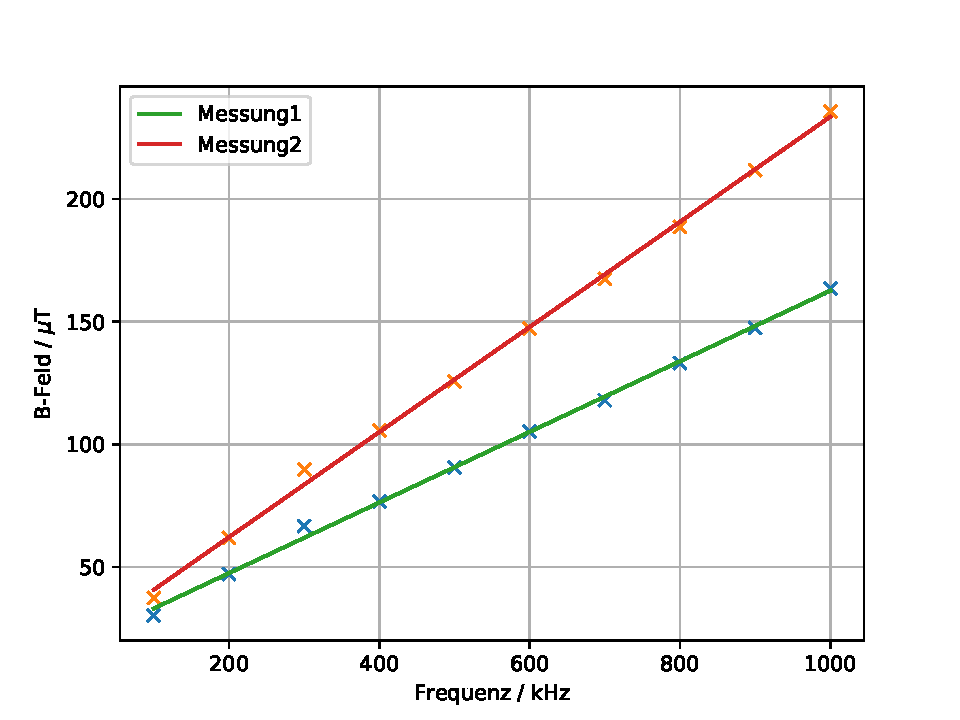
\includegraphics[width=0.8\textwidth]{B-Feld.pdf}
  \caption{Das für die Resonanzstelle benötigte Magnetfeld aufgetragen auf die Frequenz}
  \label{fig:Bf}
\end{figure}
Es wird eine Ausgleichsrechnung der Form:
\begin{align*}
  B(f)=af+b
\end{align*}
durchgeführt.
\begin{align*}
  B1&\\
  a_1&=\SI{1.438\pm 0.023e-10}{\frac{T}{Hz}}\\
  b_1&=\SI{1.876\pm 0.144e-5}{T}
\end{align*}
\begin{align*}
  B2&\\
  a_2&=\SI{2.141\pm0.031e-10}{\frac{T}{Hz}}\\
  b_2&=\SI{1.935\pm0.190e-5}{T}
\end{align*}
\FloatBarrier
Mit der Steigung $a$ kann der Landesche $g_F$-Faktor wie folgt bestimmt werden.
\begin{align*}
  g_F = \frac{h}{\mu_0\cdot a_i}
\end{align*}
Somit ergeben sich die Landeschen Faktoren zu:
\begin{align*}
  g_{F1} = 0,497\pm0,008\\
  g_{F2} = 0,334\pm0,004.
\end{align*}

Nun soll der Kernspinn bestimmt werden.
Dieser kann mit der Formel:
\begin{align*}
  I = \frac{1}{2}\left(\frac{g_J}{g_F}-1\right)
\end{align*}
berechnet werde.
Das benötigte $g_J$ kann wie folgt bestimmt werden.
\begin{align*}
  g_J = \frac{(g_s+1)\cdot J\cdot(J+1)+(g_s-1)\cdot[S\cdot (S+1)-L\cdot (L+1)]}{2\cdot J \cdot (J+1)}
\end{align*}
Dabei ist $g_s$ gegeben als
\begin{align*}
  g_s = 2,0023
\end{align*}
Durch einsetzen der gegebenen Quantenzalen, welche in dem Versuch sind gegebnen als
\begin{align*}
  S = \frac{1}{2}, L=0, J=\frac{1}{2}, F = I+J
\end{align*}
Läst sich die relation aufstellen:
\begin{align*}
  g_J=g_s.
\end{align*}

Der Kernspinn kann jetzt bestimmt weren.
\begin{align*}
  I_1=1,5153\pm0,03\\
  I_2=2,4999\pm0,04
\end{align*}
Durch einen Vergleich mit Literaturwerten kann der Kernspinn den Rubidium-Isotopen zugeortnen werden.
Es gilt:
\begin{align*}
  I_{\text{Rb85}}=\frac{5}{2}\\
  I_{\text{Rb87}}=\frac{3}{2}
\end{align*}
Es wird deutlich, dass
\begin{align*}
  I_1=I_{\text{Rb87}}\\
  I_2=I_{\text{Rb85}}
\end{align*}
gilt.

Mit Hilfe der Formel \ref{eqn:quadzeeman} kann die Wechselwirkungsenergie der Hyperfeinstrucktur bestimmt werden.
Die Errechneten Weren sind in der Tabelle \ref{tab.QZ} für die beiden Isotope aufgefürt.
\begin{table}
  \centering
  \caption{Der Quadratische Zeemaneffekt zu den beiden Isotopen}
  \label{tab.QZ}
    \begin{tabular}{c c c c c}
      \toprule
      Frequenz  &  B-Feld 1 & Quad. Zeeman  & B-Feld 2  &Quad. Zeeman\\
      kHz & $\mu$T & 1$\cdot10^{-20}$ & $\mu$T  & 1$\cdot10^{-20}$ \\
      \midrule
      \midrule
      100     &   30,234 &  -1,271\pm0,021   &  37,476  &   -1,998\pm0,029     \\
      200     &   47,117 &  -3,099\pm0,050   &  61,902  &   -5,464\pm0,078     \\
      300     &   66,680 &  -6,219\pm0,100   &  89,733  &  -11,491\pm0,164     \\
      400     &   76,757 &  -8,246\pm0,133   & 105,724  &  -15,957\pm0,228     \\
      500     &   90,587 & -11,493\pm0,185   & 125,769  &  -22,587\pm0,323     \\
      600     &  105,093 & -15,477\pm0,250   & 147,069  &  -30,891\pm0,442     \\
      700     &  117,982 & -19,512\pm0,315   & 167,429  &  -40,041\pm0,573     \\
      800     &  133,105 & -24,843\pm0,401   & 188,631  &  -50,829\pm0,727     \\
      900     &  147,574 & -30,545\pm0,493   & 211,730  &  -64,047\pm0,916     \\
      1000    &  163,518 & -37,510\pm0,605   & 235,565  &  -79,284\pm0,113     \\
      \bottomrule
    \end{tabular}
\end{table}

